\chapter{DevArtist}
\label{ch:devartist}
The prototype presented here is a hybrid tool which combines both static and dynamic analysis leveraging what \emph{ARTist} offers, by creating a module which checks and patches: the usage of insecure random, the execution of insecure queries and the usage of known broken hashing algorithms. Specifically, \emph{DevArtist} looks for the signature of the methods introduced in chapter \ref{ch:investigation} at compile-time and uses an auxiliary library called \texttt{CodeLib} to check and patch the aforementioned issues.

\section{Design Goals}
Before introducing \emph{DevArtist}, it is necessary to define the properties which an ideal tool should have to tackle the problem of vulnerable apps, most characteristics that follows are derived from existing approaches.
\begin{itemize}
	\item{Diminish the attack surface of the app: an attacker should have a harder time exploiting it, to obtain information about the user.}
	\item{Avoid extra work for developers: a plug and play system which patches the security issues they left open and does not require any code to be set-up. Although preventing developers to write insecure code in the first place would be a better approach, the option we choose takes into the account the fact that there are already published apps, which would need to be, otherwise, re-written.}
	\item{Avoid making the app more likely to dysfunction: It is important that the system keeps intact the original reliability and stability without impeding the normal usage of the apps.}
\end{itemize}

\section{Deployment}
In the following sections are discussed the deployment options for \emph{DevArtist} and it is stated which benefits each solution brings to users and at what cost. 

\subsection{As Default Compiler}
\label{sc:deploy}
A possibility for \emph{DevArtist} is to become the default compiler in a forked version of Android (commonly called ROMs) and ship directly within it, by replacing the original dex2oat. The end-users would incredibly benefit by this change, due to the fact that all user-installed applications would go through the improved process of compilation, providing extra security. Shipping \emph{DevArtist} within a security focused ROM is not an impossible task since such projects already exists. One example, is CopperheadOS\footnote{\url{https://copperhead.co/android/}} which wants to provide an hardened version of Android to people concerned about privacy. Although merging the two projects would increase the overall security of the resulting OS and would not make the end-users choose between the security models offered by CopperOS and this work, it might still be too hard for an average user to really take advantage of the possibility, due to technical level of knowledge required to install a custom ROM. In addition to the difficulty, many device manufacturers explicitly forbid unlocking the boot-loader by voiding the warranty when an unlocked device is sent for reparations. Especially for the latter reason and for the fact that the OS change requires wiping a device data, which would decrease the effort of supporting end-users, this deployment option is not the one chosen for \emph{DevArtist}.

\subsection{As Application}
\emph{DevArtist} can be delivered to end-users as a normal application, which can be downloaded from the Play Store and used to re-compile all the applications that the user deems as needing. At first glance, this option seems the most promising due to the fact that it does not require extra knowledge from users but it also implies root permissions. In fact, to achieve this goal, it is necessary to ship our modified dex2oat within \emph{ArtistGUI} (\emph{DevArtistGUI} from now on), which then needs to replace the original OAT file with the instrumented one. However, the original OAT File is located in a folder protected by OS (fortunately for the user but unfortunately for our purposes), thus requiring elevated privileges. Despite this problem, which is discussed further on, this is the path taken by this project. The choice does not require wiping the data or voiding the warranty of a device, making it a better option to show the potential of this prototype to end-users.

\section{Use Cases}
Despite the tool's focus on end-users and taking into account its prototypical stage, there are several other ways in which the system can be used, depending on the agent. In fact, changing the perspective sheds lights on possible scenarios, which are worth discussing. 

\subsection{Company (or Solo Developer) Use Case}
From the perspective of a company, using \emph{DevArtist} is useful as vulnerability scanner to deliver a more secure apk. The goal can be achieved by using the tool internally to re-compile and check the log produced by this system and learn about the pitfalls that are in the code. In fact, \emph{DevArtist} logs all the patches that are applied during runtime, hence a developer only needs to read the output of the Logcat while running the app, to learn what's wrong and avoid making the same mistake in the future. In addition, thanks to the flexibility of the system and its open-source license, a company might decide to extend this tool to publish a full featured application, which harden even more Android devices. It is worth to mention that all these possibilities also apply to a singular developer.

\subsection{Security Researcher Use Case}
\emph{DevArtist} enables researchers to compute statistics and benchmarks over the vulnerabilities it already covers. Moreover, \emph{DevArtist} can be a better building block than \emph{Artist} itself, when there is the need of extending the platform by adding or removing a few vulnerability checks. However, the current state of \emph{DevArtist} (or \emph{Artist}), does not include a structure allowing to define what a vulnerability is and how to patch one when encountered by the system, but this behavior must be coded directly into the module. This is a limitation that future work might solve, improving greatly the usability for this use case.

\subsection{End User Use Case}
This is the case on which this thesis focuses the most, due to the fact that an end-user can install the apk of \emph{DevArtistGUI} and make it compile all the applications it wants to gain extra security for. However, the need of enabled root permissions on the device poses a threat to their security and it limits the adoption of this solution. In fact, rooting options are not available for every Android device and, for the remaining part, the procedure is seen as complicated nonetheless dangerous, due to the fact that it voids the warranty for many devices. However, by looking at the official dashboard page of Android at \cite{anddash}, device manufacturers often choose to not update their devices with the latest version of Android at all or in a timely manner, hence the 63\%\cite{muchroot} of Android users claim to gain root privileges in order to update their devices through a custom ROM\footnote{Unofficial distributions of Android, created by third party developers}. With such a significant share of rooted devices, the task of dropping the root requirement becomes minor and it is left for further research. 

\section{On Abusing DevArtist}
As a matter of fact, it is worth to consider the possibility that \emph{DevArtist} falls in the hand of a misguided \enquote{security researcher}. In this case, the tool can be abused as a vulnerability scanner to analyze which pitfalls are in an application and exploit that information to mount an attack. Consequently, a na\"ive way to make this scenario harder is excluding from \emph{DevArtistGUI} the logs of what it has patched, such that an attacker would have to add the code themself and re-compile both the module for \textbf{dex2oat} and \emph{DevArtistGUI}. However, this solution would have two main problems: the first is that it would make the tool less usable from the perspective of the first use case and, on the other hand, it actually does not solve the problem for a resolute attacker who decides to go the long way and it's not concerned of the extra effort. This is a problem, somewhat philosophical, that many research in the security field have, but the only solution available is that all the works in this area, including this one, hopefully will increase the awareness of security issues and will improve the overall environment.

\section{Taxonomy}
It is necessary to divide the patches that follows in two categories: \textbf{safe} and \textbf{risky}.
A patch is considered \enquote{safe} whenever its implementation does not interfere with the behavior of the compiled app: not making it more likely to crash or, worse, unusable. It's worth to mention that to really test if the following patches can be considered \enquote{safe}, the evaluation part includes benchmarks targeting especially this definition. On the other hand, \enquote{risky} means the opposite definition: the patch contains an algorithm that might corrupt some functionality of the targeted app, inducing it to crash more often or other unwanted and not foreseeable behavior.


\section{Unsafe Queries}

Patching unsafe queries was the hardest part to code and the algorithm is pretty long due to the fact that it must find what composes the final sql string executed by \textbf{rawQuery}. Hence, I will split the algorithm in two parts and highlight only those. In addition, to make the reading easier, these two parts are being named: \textbf{searchTaint} and \textbf{searchUses}. Moreover, the reader can find an example of the underlying IR in figure \ref{fig:querygraph}, to follow along with the algorithms.

\subsection{Overview}
The main idea behind solving the \emph{rawQuery} problem is to find the parts of the query which are not hard-coded and assume the rest untrusted. Moreover, the algorithms checks if the query is a pre-loaded string, or it is composed with a \textbf{StringBuilder}. In the first case, the query is considered safe because the string is provided by the developer itself, whilst in the other case it looks for all the parts in the backward slice of the method. In fact, starting from \emph{rawQuery} until the method \textbf{NewInstance} of the StringBuilder is found, the whole string can be re-constructed and every instruction which is not of type \textbf{LoadString} (which indicates hard-coded strings) is considered as a tainted value to be included in the tainted set.
Afterwards, the call to the \emph{rawQuery} method is replaced with the call to a function contained in the \textbf{CodeLib}, namely \texttt{patchedRawQuery()}, which takes as inputs all the inputs of the original one but with the addition of the tainted set. From here, the new method checks at runtime every variable in the tainted set by comparing with common SQL injection strings and, if an injection is found, that part gets removed.

\begin{figure}
	\centering
	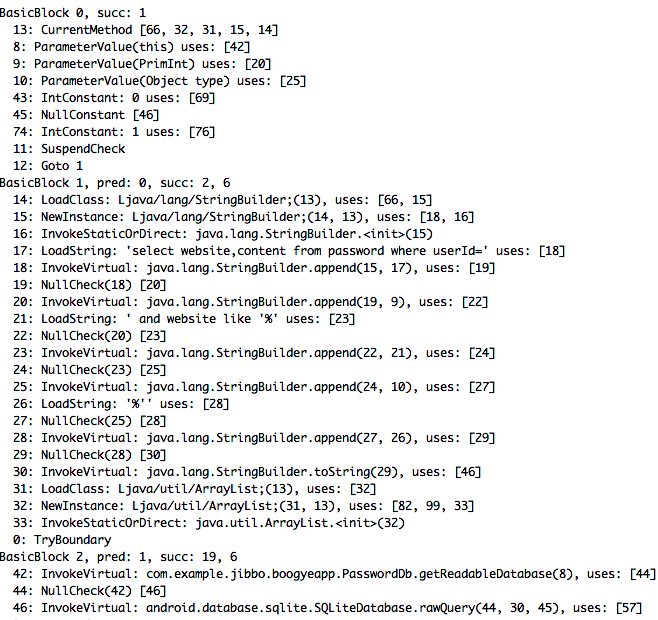
\includegraphics[scale=0.7]{img/query_graph.png}
	\caption{unsafe query example of IR, in its string representation}
    \label{fig:querygraph}
\end{figure}
\newpage
\subsection{Execution of SearchTaint}
This algorithm is used to find the source of every StringBuilder. The process starts after the visitor (check section \ref{sec:artist} for reference) finds the \textbf{rawQuery} method: our code checks if the SQL string is composed within a \texttt{StringBuilder} and, if yes, this part of the algorithm is called upon \texttt{StringBuilder.toString()}. Fundamentally, \textbf{searchTaint} computes the backward slice of the before mentioned instruction and while its computing, it also checks the kind of every instruction: if it is a ParamValue, the instruction is added to the tainted set, whilst: if it is instead either LoadString or ConstantValue it stops because they are hard-coded (meaning trusted), otherwise it continues by re-calling itself upon every input of the instructions. Moreover, the algorithm also calls \texttt{searchUse} whenever the instantiation of a StringBuilder is found, this is done to be sure that every usage of the StringBuilder are covered. However, due to its implementation, \emph{Artist} cannot pass arrays to the \textbf{CodeLib}, where the \emph{patchedRawQuery} resides, hence the additions to the tainted set is done by injecting a method, which code resides in the auxiliary library, and passing only the tainted instruction as a parameter to that. Listing \ref{alg:sqlcompsearchinputs} shows the code for this first part of the algorithm.

\begin{algorithm}
\caption{Checking the StringBuilder Backward Slice}
\label{alg:sqlcompsearchinputs}
\begin{algorithmic}[1]
\Procedure{searchTaint}{}
\State $\textit{Node} \gets \text{instruction containing the final query}$
\State $\textit{Graph} \gets \text{The graph containing all the instructions of this block}$
\If{$\text{node \textbf{not in} } \textit{alreadyChecked}}$
	\State $\text{alreadyChecked.add(node)}$
	\If{$\text{node.getKind() \textbf{is}}\textit{NewInstance}}$
		\State $\text{// It's a StringBuilder instantiation}$
		\State $\text{searchUses(node,graph)}$
	\ElsIf{$\text{node.getKind() \textbf{is} }\textit{LoadString or ConstantValue}}$
		\State $\text{// It's safe, we just stop}$
		\State $\text{alreadyChecked.add(node)}$
	\ElsIf{$\text{node.getKind() \textbf{is} }\textit{ParamValue}}$
		\State $\textit{Graph} \gets \text{injectAddToTaintedSet(node)}$
		\State $\text{alreadyChecked.add(node)}$
	\ElsIf{$\text{node.inputCount()} > \text{0}}$
		\State $\text{// It's a NullCheck or an InvokeVirtual}$
		\State $\text{alreadyChecked.add(node)}$
		\For{$i \gets 1 \textrm{ to } node.InputCount()$}
	        \State $\text{searchTaint(node.ChildAt(i),graph)}$
	     \EndFor
	\EndIf
\EndIf
\EndProcedure
\end{algorithmic}
\end{algorithm}


 % All the components are added to the tainted set and this method ends when the algorithm finds all the instantiations of the \textbf{StringBuilder}s themselves, thus calling the second part\footnote{All the hard-coded strings which compose the final sql string are considered safe and not added to the tainted set}. Therefore, \textbf{SqlCompSearchUses} checks that the usages of the string builder and calls \textbf{SqlCompSearchInputs} for every use which wasn't already visited\footnote{The algorithm offers, of course, margins for optimization in both memory and speed, although I preferred to leave the prototype easier to understand to better aid future modifications.}. The tainted set, then gets sent to the support library which code is merged in to the app and that will check at runtime if the query components are tainted and, in the case it might contain an injection, it will prevent its execution. The code of the library can be considered a streamlined version of dynamic analysis. In fact, it scans, at runtime, what is contained in the user inputs and compares it to an hard-coded array of common sql attack vectors. The algorithms that follows are the pseudo-code representation of the above mentioned parts, the library code is omitted for brevity given its simplicity. 

\subsection{Execution of SearchUses}
This part of the algorithm gets called when a StringBuilder is instantiated by the call \texttt{NewInstance: java.lang.StringBuilder} and it checks every usage of the builder \texttt{searchTaint}, to ensure that none is omitted. When one of those instruction is found, the first part of the algorithm is called again on that to check whether is a trusted one or untrusted. Listing \ref{alg:sqlcompsearchuse} shows the code for this part of the algorithm.

\begin{algorithm}
\caption{Checking the StringBuilder Usages}
\label{alg:sqlcompsearchuse}
\begin{algorithmic}[1]
\Procedure{searchUses}{}
\State $\textit{Node} \gets \text{instruction containing }\textit{android.database.sqlite.SQLiteDatabase.rawQuery}$
\State $\textit{Graph} \gets \text{The graph containing all the instructions}$
\If{$\text{node \textbf{not in} } \textit{alreadyChecked}}$
	\State $\text{alreadyChecked.add(node)}$
	\If{$\text{node.getName() \textbf{contains not} }\textit{"init"}}$
		\State $\text{searchTaint(node,graph)}$
	\ElsIf{$\text{node.usesCount()} > \text{0}}$
		\State $\text{// It means we still haven't arrived}$
		\State $\text{searchUses(node,graph)}$
	\EndIf
\EndIf
\EndProcedure
\end{algorithmic}
\end{algorithm}

\subsection{The Codelib}
The last piece of the algorithm checks every component sent in the compilation phase by \texttt{searchTaint} and checks at runtime the content of the variables against a static vector of common SQL injection strings. All the tainted components of the query are removed from it before it is executed on the database. Moreover, if no component is flagged as an injection, the algorithm tries to look on the full query for parts that contains at least one of the common injections methods listed in the static vector and, only after nothing is found, the query is executed. The code for this check is trivial due to being mostly only a string comparison. Hence is not reported.

\subsection{Limitations of the Approach}
The hard-coded array contained in \textbf{CodeLib} might represent a point of failure due to the fact that it cannot be comprehensive of all the possible sql injections. However, on Android, prepared statements do not return a resulting cursor and calling the other methods, where safety is achieved by letting the framework compose the query, will require to implement a full-fledged SQL parser. Moreover, despite JSqlParser\footnote{\url{https://github.com/JSQLParser/JSqlParser}}, whose usage has been tested and validated and it was not flexible enough for the goal our prototype needed, the shortage of parsing libraries made impossible, in the constraint of this thesis, to develop a better solution. Further development of this work should tackle this problem and provide a better solution. Escaping is also a viable approach and it was taken into account in the design phase but, using this technique would break the functionalities of all those applications that allow querying directly a database, hence discarded.

\section{Randomness}
The algorithm to replace insecure random usage might seem easy at first. In fact, intuitively, it should be enough to replace the call \texttt{new Random()} with the secure one: \texttt{new SecureRandom()}. However, \emph{ARTist} does not provide a callback to its modules when an instruction of type \texttt{NewInstance} is found. Therefore, in order to patch this, the module needs to wait for the callback that get triggered when the method \texttt{java.util.Random.<init>} is found and then execute a smaller DFS inside the whole block containing the backward slice of this line to find the new instance and replace it. The pseudo-code is as follows:
\begin{algorithm}
\caption{Random patching}\label{euclid}
\begin{algorithmic}[1]
\Procedure{patchRandom}{}
\State $\textit{instruction} \gets \text{instruction containing }\textit{java.util.Random.init}$
\State $\text{randomInstruction} \gets \text{instruction.getBlock().getFirstInstruction()}$
\While{$\text{randomInstruction \textbf{is not} } \textit{null}}$
	\If{$\text{randomInstruction.getKind()} ==  \textit{NewInstance}}$
		\State $\text{debugName} \gets \text{getSignature(randomInstruction)}$
		\If{$\text{debugName contains } \textit{java.util.Random}}$
			\State $\text{brake; // found, go on with the part after this while}$
		\EndIf
	\EndIf
	\State $\text{randomInstruction} \gets \text{randomInstruction.getNext() // will return null at the end}$
\EndWhile
\If{$\text{randomInstruction \textbf{is not} } \textit{null}}$
		\State $\text{injection} \gets \text{injectSafeRandomInstance()}$
		\ForAll{$\text{use} \gets \text{randomInstruction.getUses()}}$
			\State $\text{use} \gets \text{replaceInput(0,injection) // input 0 is the instance of the random}$
		\EndFor
\EndIf
\EndProcedure
\end{algorithmic}
\end{algorithm}

\subsection{Limitations of the Approach}
Given the nature of random number generators, the functionalities offered by an application are not compromised when one is used instead of another (in the end both should output numbers that look random from the outside), but this holds true only when swapping one algorithm for a more secure one. As already explained in section \ref{sec:randominvestigation}, this is the case in our algorithm and, although there is no perceivable difference between the output of the two when used inside an application, it should also hold true from a user perspective. In fact, unless a developer is exploiting the weaknesses of the class Random explicitly, an end user should not notice any difference in the behavior of the program. Moreover, since it can be assumed that the everyday user cannot tell the difference between two numbers obtained from two different generators, the only way they can notice the algorithm swap is when a significant decrease in performance takes place. On this regard, the documentation published by Oracle only states that \texttt{SecureRandom} has to wait, before returning a value, until enough entropy is available and the official Android one does not mention differences in execution speed between the afore-mentioned class and \texttt{Random}. For this purpose, I developed an app, which code is available on Github\footnote{https://www.github.com/jibbo/master\_thesis}, to test their performances. The app was executed multiple times on a low-end device such as the Kindle Fire (7 inches model, 2017 version), which has a 1.3Ghz arm quad-core processor from Mediatek and it has been rebooted before each execution of the test. \texttt{Random} was generating an Integer number instantly, whilst \texttt{SecureRandom} took, on average, 1ms. Although this test needs to be run on a larger scale, it suggests that on similar hardware there is a small decrease of performance. However, a 1ms delay is not perceivable by users, hence replacing Randomness can be considered a safe patch which only improves security.

\section{Hashing}
As already discussed in chapter \ref{ch:investigation}, MD5 and SHA1 have been proven to be broken. However, they are still widespread among app developers to verify the integrity of packages or for other needs. What the module does in this case, is replacing the algorithm name when invoking the instance of \texttt{MessageDigest} with SHA-256.

\begin{algorithm}
\caption{Hashing patching}\label{euclid}
\begin{algorithmic}[1]
\Procedure{patchHash}{}
\State $\textit{instruction} \gets \text{instruction containing }\textit{java.security.MessageDigest.getInstance}$
\State $\textit{safeAlgName} \gets \text{"SHA-256"}$
\State $\text{instruction.InputAt(1)} \gets \text{safeAlgName}$
\EndProcedure
\end{algorithmic}
\end{algorithm}

\subsection{Limitations of the Approach}
Despite the simplicity of the modification, changing the algorithm used for hashing is very delicate and might break functionality. This contrasts the third characteristic of an ideal tool and this is why this patch is considered "Risky". In particular, the dysfunction happens all the times that an external part of an application architecture, which \emph{DevArtist} is unaware of, does not support the new hashing algorithm. For example: an application that downloads and verifies an add-on via MD5 and, if the hash matches with the one specified by the server, it enables the add-on, otherwise it triggers the download again. In this case, the proposed solution breaks the integrity check due to the algorithm mismatch between application and server, producing an unusable application by keeping it in the verification (plus download) loop for a long time and eventually making it crash as soon as the maximum amount of resources allocated for the process ends.

\section{Debating the Usefulness of DevArtist}
In the previous chapter are described the reasons why patching these vulnerabilities is a necessity, but it is worth to mention that not all the signatures found by \emph{DevArtist} can be exploitable by an attacker, such as, for example, it can be a SQLi injection in a query which is never executed. Moreover, the proposed fixes cannot patch vulnerabilities completely in all the cases and this, united with the example just mentioned and the fact that risky patches reduces the functionality of an app, question the usefulness of \emph{DevArtist}. However, as already mentioned in this work, it is important to see \emph{DevArtist} in its context, which is the one of a prototype not yet suitable for the masses but only for security focused environments and privacy concerned experimenters. Therefore, for this niche, hardening the most of a system is not only important but better due to the fact that it improves the overall security by making the whole environment less prone to attacks. In addition, project such as F-Droid\footnote{\url{https://f-droid.org}}, which is an open-source market for apps, show that patches which break application functionalities do not limit considerably the number of this particular subset of users, due to the fact that they are accustomed to use less apps, provided that the ones that work are perceived as more secure.

 
